%% report_template.tex
%% V1.0
%% 2012-03-16
%% by Jesper Pedersen Notander
%% See:
%% http://www.cs.lth.se/jesper_pedersen_notander
%% for current contact information.
%%
%% This is a template file contaning instructions and a skeleton outline
%% for the final report in the course ETSA05: Software Engineering
%% Process - Soft Issues, given by the Department of Computer Science at
%% Lund University, Sweden.
%%
%% This template requires IEEEtran.cls, written by Michael Shell, version
%% 1.7 or later.
%%
%% Support sites:
%% http://www.cs.lth.se/etsa05/
%% http://www.ieee.org/

%%*************************************************************************
%% Legal Notice:
%% This code is offered as-is without any warranty either expressed or
%% implied; without even the implied warranty of MERCHANTABILITY or
%% FITNESS FOR A PARTICULAR PURPOSE!
%%
%% User assumes all risk.
%%
%% In no event shall Lund University or any contributor to this code be
%% liable for any damages or losses, including, but not limited to,
%% incidental, consequential, or any other damages, resulting from the use
%% or misuse of any information contained here.
%%
%% All comments are the opinions of their respective authors and are not
%% necessarily endorsed by Lund University.
%%
%% This work is distributed under the LaTeX Project Public License (LPPL)
%% ( http://www.latex-project.org/ ) version 1.3, and may be freely used,
%% distributed and modified. A copy of the LPPL, version 1.3, is included
%% in the base LaTeX documentation of all distributions of LaTeX released
%% 2003/12/01 or later.
%%
%% Retain all contribution notices and credits.
%% ** Modified files should be clearly indicated as such, including  **
%% ** renaming them and changing author support contact information. **
%%
%% File list of work: report_template.tex
%%*************************************************************************


\documentclass[conference]{IEEEtran}
\usepackage{graphicx}
% If IEEEtran.cls has not been installed into the LaTeX system files,
% manually specify the path to it like:
% \documentclass[conference]{../sty/IEEEtran}

\begin{document}

\title{On the Design of Software Processes and Software Process Improvement in
the Context of Lego Scrum Workshops}

% Leave as is to ensure anonymous grading.
\author{
\IEEEauthorblockN{ANONYMOUS AUTHOR}
\IEEEauthorblockA{Examination in DIT348 Software Development Methodologies\\
Department of Computer Science and Engineering\\
University of Gothenburg\\
Gothenburg, Sweden}}

\maketitle

\begin{abstract}
This paper discusses the design of a software process in the context of Lego
Scrum workshops as part of the course DIT348 Software Development Methodologies
offered by Gothenburg University (Sweden). Subsequently, the paper provides
insights about software process improvement (SPI) techniques and proposes an
SPI initiative with a redesigned process (accompanied with a SPEM 2.0 diagram).
Ultimately, the paper discusses various challenges that practitioners encounter
when conducting SPI efforts, and provides an additional insight into the
feasibility of the Scrum of Scrums methodology.
\end{abstract}

\section{Introduction}

% The introduction section should be used to introduce Software Processes and
% Software Process Improvement (SPI) in general and to introduce the purpose
% and context of this report.

A software process is a goal-oriented approach which incorporates a set of
tools, methods, and practices to produce a software product or a more general
software service \cite{Munch2012}, \cite{Humphrey1989}. With the increasing
complexity of software systems, the need for a well-defined software process
has become more and more significant. Basili and Rombach \cite{Basili1988}
state that software engineering processes require \textbf{tailorability}
because of the diversity of the software products and the different
environments in which they are developed, hence the need for a software process
improvement (hereafter SPI) initiative.

This paper analyzes a designed software process and proposes an SPI
initiative---based on which the process is to be improved---in the context of
the Lego Scrum workshops. The text is complemented with knowledge and
experiences from peer-reviewed literature and the course material alongside
several research studies are conducted by the frontiers of the software
engineering field (e.g., \cite{Basili1988}, \cite{Caldiera1994},
\cite{Schwaber2020}).

\section{Process Defined for the Scrum Workshop}
\label{sec:process}

% Describe the process you defined for the Scrum Lego Workshop. Explain whether
% you chose to apply Scrum, User Story Practice, and Incremental Delivery. Give
% reasons for why you did or did not use elements from these three practices.

The defined process is titled {\fontfamily{qhv}\selectfont AKAMMO} and
utilizes concepts from Scrum, Incremental Delivery, and, to a lesser extent,
User Story Practice \cite{DIT348A1}. Scrum provides a flexible and adaptive
approach to project management and encourages transparency in terms of the
project's progress and the issues encountered \cite{Schwaber2020}. Scrum, by
definition, is meant to be applied in an iterative manner, which is why a
conjunction with Incremental Delivery becomes a natural choice
\cite{Schwaber2020}, \cite{Srivastava2017}, \cite{Schwaber1997}.

Initially, the process assumes a set of user stories that are to be implemented
(and are prioritized by the Product Owner [hereafter PO]). Afterwards, the team
members analyze the user stories and decide whether they require a further
elicitation of requirements (which is discussed with the PO) or whether they
can be implemented as they are.
Moreover, at the beginning of each sprint, \textbf{sprint planning} takes
place. It is an activity that aims to split up the user stories into more
granular requirements, where each requirement is accompanied with a set of
acceptance criteria. The requirements are then assigned to the members of
the team---the delegation of requirements is carried out in a way that the team
members have agreed upon, although, in case of a disagreement, round-robin,
random choice, or any other method can be used. 

Subsequently, the requirements are assigned \textbf{story points} that
correspond to the difficulty of their implementation (i.e., the higher
the number, the more difficult the implementation) based on the Fibonacci
sequence. Strikingly, Tamrakar and J\o{}rgensen \cite{Tamrakar2012} note that
the Fibonacci scale, along with other non-linear scales, eliminates a bias
present in linear scales, where individuals tend to favor the middle.
Consequently, non-linear scales yield more accurate results.

Furthermore, a \textbf{Kanban board} is used throughout the workshop to
categorize each requirement into following columns: (i) \textit{To Do}, (ii)
\textit{In Progress}, (iii) \textit{Done}. The reason why a Kanban board was
considered to be a part of the process can be supported by a claim made by
Ahmad et al. \cite{Ahmad2014} suggesting that a Kanban board provides
visibility to a [software] development process, communicates priorities, and
highlights bottlenecks. However, no specific type of the board is
assumed---physical or digital boards are equally viable.

What's more, a sprint lasts an hour, and as the end of the sprint approaches, a
meeting, which combines a sprint review and a sprint retrospective, is held
(adapted from Scrum \cite{Schwaber2020}). During the meeting, the team
discusses difficulties they encountered and evaluates the overall progress
carried out. Additionally, this meeting should yield an \textbf{increment}
which the team has produced over the course of the sprint. It is, afterwards,
delivered to the PO once the meeting has concluded.

The process, by default, does not schedule any breaks; however, there is a
possibility of a so-called \textit{"emergency break"} which can be called by any
team member at most once every 30 minutes. Breaks on an individual basis are
allowed, but should not interfere with the team's progress. In a typical Scrum
environment, stand-up meetings are held repeatedly and last for a short period,
e.g., 15 minutes \cite{Schwaber2020}. However, in the context of the Lego Scrum
workshop, the team is not obliged to hold such meetings, because merely six
members are involved in the team, and the workshop is not meant to last longer
than four hours.

\section{Experiences in the Scrum Workshop}
\label{sec:experiences}

% In this section, you should describe your experiences during the first Scrum
% Lego workshop. Put a special focus on how you and your group were using the
% process, which parts of the process worked well, and which parts of the
% process did not work well. For the latter part, analyze the reasons that
% caused problems. Use at least three references to the literature (e.g.,
% \cite{CaterSteel2006}, \cite{Abrahamsson2002}) to identify if the issues you
% encountered are general problems or specific to your effort.

On the whole, the designed process, {\fontfamily{qhv}\selectfont AKAMMO},
was a viable choice for the first Lego Scrum Workshop. The team members perceived
it as flexible enough to accommodate the needs of the team, while not being too
rigid to hinder the team's progress \cite{DIT348A2}.

The process has been followed in the desired manner (described in
Section~\ref{sec:process}) with very few deviations. The process has
been made use of for the first time, allowing the team to identify shortcomings
(that are addressed in the following subsections) propose improvements, and
highlight successful aspects. 

Firstly, the team members agreed that initiating a sprint with a \textbf{sprint
planning} enabled them to have a clear understanding of the requirements that
were to be worked on. Secondly, it was observed that merging the sprint review
and retrospective into a \textbf{single meeting} was a logical choice. Usually,
these meetings briefly covered team difficulties and progress, hence no need to
separate them into two meetings. Omitting stand-up meetings was considered
reasonable due to the small team size (six members), the short duration of the
workshop (not exceeding four hours), and seamless communication among
participants, because all were present in the same room. Remarkably, our
process, influenced by the points mentioned above, proved highly effective,
with no team member calling for \textit{"emergency breaks"}.

However, team members identified various concerns which are explored in the
following subsections with references to relevant literature. Firstly, a lack
of a sensible \textbf{Definition of Done} (abbreviated as DoD) was observed.
Put simply, a DoD is a set of criteria points applied iteratively to each
granular increment of a product to assure that the increment is of a desired
quality when considered to be \textit{done} \cite{Kopczynska2022}. The DoD
principle is a crucial component of the product's quality assurance, and, as
Abrahamsson and Kautz \cite{Abrahamsson2002} point out, quality assurance
entails an ability to identify defects as early as possible---this becomes
viably achievable with a well-defined DoD.

The absence of a Definition of Done (DoD) can lead to an undesirable product
quality and increased development costs. Additionally, it may cause
misunderstandings between team members and the PO, hampering overall project
progress. These (and other) observations are based on a study conducted by
Kopczynska et al. \cite{Kopczynska2022}.

Furthermore, during the second and the third sprints, the team \textbf{omitted
assigning story points} to user stories. This stemmed from team members being
deeply engaged in working on individual user stories, leading them to skip
assigning story points. Undeniably, this might lead to a serious threat in a
real-word project. As Abrahamsson and Kautz \cite{Abrahamsson2002} observe, it
is a recurring issue that teams conduct improper estimations---in our case, the
estimations were not made at all. The absence of estimations, especially in the
face of serious risks, would complicate and, in some cases, make it impossible
to evaluate the impact on the project's progress.

Lastly, it has been observed that the process did not mention any
\textbf{cross-team communication efforts}. However, the nature of the Lego
Scrum workshop was to produce a city environment with a set of buildings, where
each team was responsible for one (or more) buildings. It is, in this case,
unavoidable that the buildings are interconnected in some way, and, as a
result, the teams were required to communicate with each other. This fact was
not taken into account when designing the process and proved to be a bottleneck
for the team's progress. This is, in fact, not an issue specific to our
endeavor, albeit a rather general problem. Larsson and Larsson
\cite{Larsson2020} postulate that conducting cross-team collaborative
approaches to lessen integration risks is unavoidable, and should not be
disregarded in any high-quality process. Cater-Steel et al.
\cite{CaterSteel2006} further emphasize the importance of cross-team
communication by stating, quote, \textit{"[...] high quality external expertise
is more critical than top management support."} It is thereby evident that the
lack of cross-team communication poses a serious threat which should be
addressed if the process is to be used in the future iterations of the
workshop.

\begin{figure*}
	\centering
	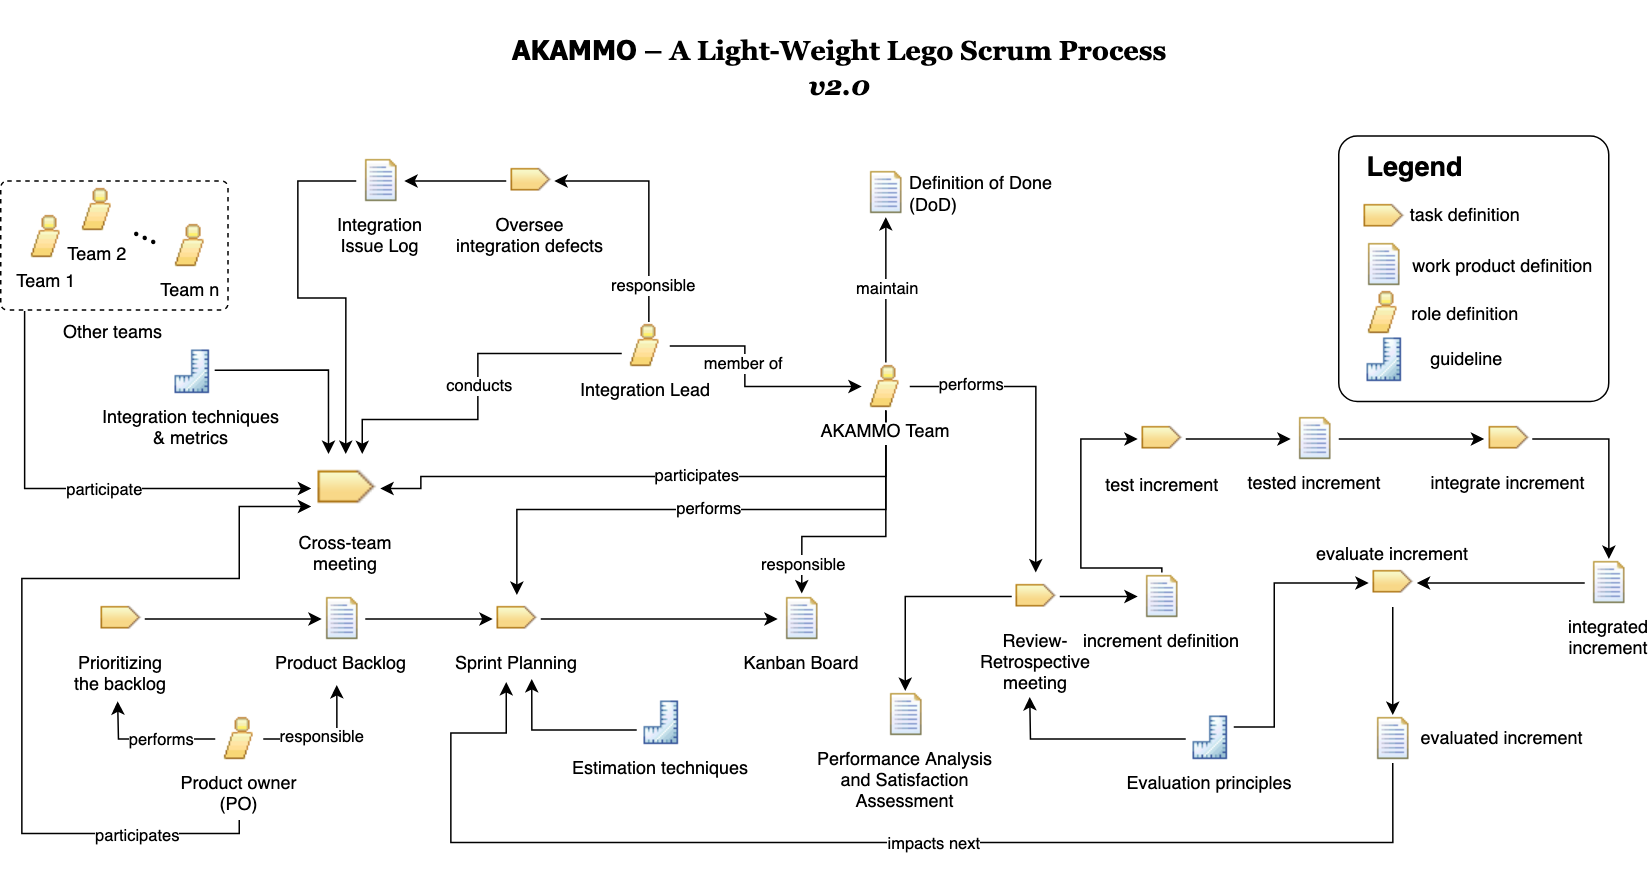
\includegraphics[width=0.9\textwidth]{process-diagram.png}
  \caption{SPEM 2.0 diagram of the updated process}
	\label{fig:process-diagram}
\end{figure*}

\section{Software Process Improvement Techniques}
\label{sec:spi-techniques}

% Provide at least three examples of SPI methods/models/techniques (for an
% overview, see, e.g., \cite{Pettersson2008}). Describe each of them together
% with at least one advantage and one disadvantage.

In our ever-emerging world of software, there is a plethora of SPI methods,
models, and techniques that are available to practitioners. Examples of some
common SPI models include the Capability Maturity Model Integration (CMMI), the
ISO/IEC 15504 standard, or, a more lightweight approach, the iFLAP model
\cite{Pettersson2008}. In this section, I will briefly describe some of the
techniques that are introduced by iFLAP in relation to the process that was
designed for the Lego Scrum workshop. CMMI and ISO/IEC 15504 are not discussed
in this section, since our process is merely applicable to a small-scale
project (with a defined time frame of no more than four hours). Thus, the
aforementioned models may not be suitable for our endeavor.

\textbf{{\fontfamily{qhv}\selectfont iFLAP}} is an inductive process assessment
framework that puts an emphasis on the involvement of practitioners in the
assessment process \cite{Pettersson2008}, \cite{Malvius2009}. Its core
principles are to: (i) construct a feasible selection of roles (and projects),
(ii) gather data points, document them, and \textit{triangulate} the
improvement issues by analyzing the data, and (iii) construct an improvement
plan based on the analyzed data, identify dependencies among the improvement
issues, and prioritize them. These key principles (of iFLAP) are adapted from a
summary provided by Pettersson et al. \cite{Pettersson2008}.

A central part of iFLAP is the selection of \textbf{roles} that are to be
involved in the assessment process. This way, once the analysis is completed,
the findings represent viewpoints of a broader spectrum of actors, and the
viewpoints are not limited to the team only. Having applied this technique to
our process, we would be able to obtain additional insights from, for instance,
the PO(s), the instructor(s), other teams, scrum masters, and so forth. This
would allow us to identify any shortcomings of the process from different
perspectives. Consequently, the concern discussed in
Section~\ref{sec:experiences} about the lack of cross-team communication would
naturally diminish, as the technique encourages broader communication. While
the technique itself appears rather straightforward, it does present several
limitations. The role selection is a time-consuming process and might hinder
the progress of the project. Additionally, biases and other human factors may
influence the role selection. Thus, the assessment findings may provide
unreliable outcomes.

Furthermore, iFLAP suggests to \textbf{gather data} from the selected roles
with the help of interviews or questionnaires. This would allow the team to
strengthen the process by identifying issues in a more systematic manner.
However, similar to the previous technique, the primary limitation is the time
that is required to gather the data. Interviews, on a general note, provide
valuable insights into the issues at hand, albeit they tend to be
time-consuming and tedious. Questionnaires, on the other hand, are relatively
easy and quick to conduct, but they do not provide as much detail as interviews
do. Luckily, an analysis of a questionnaire becomes feasible with the help of
automated tools or scripts that can be written by any general-purpose
programming language (e.g., Python, Julia, etc.). Nevertheless, having applied
this technique to our process, we could leverage the gathered data to enhance
the process in the future stages of its maturity. For instance, we could
identify a new strategy on how a DoD is to be modeled, or, perhaps, we could
introduce a new technique to estimate user stories.

Ultimately, iFLAP further recommends to identify \textbf{dependencies between
improvement issues}, as well as \textit{"package"} the improvement issues into
improvement areas \cite{Pettersson2008}, \cite{Malvius2009}. For instance, the
lack of a DoD is an improvement issue and corresponds to an improvement area of
\textit{quality assurance}. The identification of such dependencies allows the
team to tackle the issues in a more efficient manner. That is, if a certain
dependency is found, then a successful resolution of one issue might result in
a successful resolution of another issue, or, at least, provide an indication
of how to resolve the latter issue. This technique, under general
circumstances, is not too demanding to realize. However, an extensive domain
knowledge is required to be able to draw dependencies between the improvement
issues, and, in a larger-scale project, this becomes a challenging task
\cite{Pettersson2008}. Though, in our case, the technique is relevant and
feasible to implement---it must be, however, assumed that team members have a
sufficient understanding of the domain, so that dependencies can be drawn
between the improvement issues in a sensible manner.

% Relate each of those methods/models/techniques to the problems you
% encountered and described in Section~\ref{sec:experiences}.
% Explain whether they are applicable to your issues and why.

\section{SPI Proposal for future Scrum Development Efforts}
\label{sec:proposal}

% In this section, you should discuss and explain the concrete SPI steps that
% you suggest to take in order to improve the process you applied during the
% first Scrum Lego Workshop. First, define at least three goals for an SPI
% proposal based on what you wrote in Section~\ref{sec:experiences}. Second,
% define questions and metrics you connect to those goals.

In this section, the {\fontfamily{qhv}\selectfont GQM} tool is utilized as part
of the SPI proposal. The analysis extends the work the team conducted in the
assignments of the course, notably \cite{DIT348A3}, \cite{DIT348A4}. Basili et
al. \cite{Caldiera1994} define GQM as an approach which underscores the
importance of organizations defining their \textbf{goals}, linking them to
operational data, and establishing a framework for data interpretation in order
to \textbf{measure purposefully} their progress towards the goals. It was
originally defined to evaluate defects in a set of NASA projects
\cite{Caldiera1994}, though, over the years, it has been tailored to be
applicable to a broader spectrum of projects.

Before proceeding with the SPI initiative, let us define some notation. A goal
is written as \textit{x}). A question follows the notion Q\textit{x.y}
Similarly, a metric follows the notion M\textit{x.z}. A metric, in our context,
provides a measurement plan with a general idea of how the data is to be
collected and analyzed. In some cases, there's an example provided for the ease
of understanding.

Based on the observations made in Section~\ref{sec:experiences}, the following
goals are defined for the SPI proposal:

\begin{enumerate}
  \item Improve the clarity and consistency of task completion from the
    development team’s viewpoint.
  \item Enhance the estimation and planning with the help of story points
    from the viewpoint of the development team. 
  \item Strengthen cross-team communication and integration with a
    designated role from the development team. 
\end{enumerate}

With that in mind, 1) is accompanied with the following questions and metrics:

\begin{itemize}
  \item \textbf{Q1.1}: What is the team members' understanding the DoD?
  \item \textbf{M1.1}: Number of items in the DoD that team members share a
    common understanding of. The data would be obtained from the team members
    in a designated questionnaire -- each team member would be asked to define,
    in own words, what the items of the DoD are. Then, with the help of a
    machine learning algorithm that is able to parse human language (e.g., a
    recurrent neural network), the responses would be clustered into a set of
    groups where each group represents an overlap of the responses. The number
    of groups would correspond to the metric. In case such an algorithm is not
    available, the responses can be manually clustered into groups. The
    information would be stored on a local machine of one of the team members
    and would not be shared with any third parties. Ultimatelt, the obtained
    value should be as close to the total number of items in the DoD as
    possible.
  \item \textbf{Q1.2}: How consistently is the Definition of Done applied to
    carrying work related to user stories among the team?
  \item \textbf{M1.2}: A formulate in the following manner is to be used:
    $\frac{n_d}{n} \times 100$ (\%), where $n_d$ is the number of tasks that
    followed the DoD principles when delivered to the PO, and $n$ is the number
    of all tasks expected to be worked on within a set time frame (such as a
    sprint). In the context of the Lego Scrum workshop, it is difficult to keep
    track of how many times the DoD was applied, since the team members may
    report inaccurate data. However, in the context of a real-world software
    project, this metric can be easily obtained by observing whether the DoD
    was appended to a, say, merge request (or a pull request) that was merged into
    the \textit{main} branch of the project's repository. Nevertheless, for our case, we
    assume that the team members are honest and report accurate data.
    Subsequently, the aforementioned formula is applied and team members are
    made aware of the results. The calculations are to be stored (and
    performed) on a local machine of one of the team members. Supposing that
    each sprint is evaluted separately, the obtained values can be compared and
    an increase or decrease in the metric can be observed. Ideally, each sprint
    should yield a value of $\approx 100$. Team members are encouraged to set
    an acceptable threshold interval for the metric, say $[90, 100]$, and
    strive to achieve a value within the interval. This interval can fluctuate
    depending on the team's needs.
\end{itemize}

Secondly, 2) is accompanied with the following questions and metrics:

\begin{itemize}
  \item \textbf{Q2.1}: How accurately do the assigned user story points align
    with the actual time invested?
  \item \textbf{M2.1}:
    Decide how many minutes one story point represents (this is to be decided
    at the beginning of a sprint by all team members). For this example, let's
    say that one story point represents 5 minutes. Then, once the sprint has
    elapsed, a randomly chosen team member collects the total number of story
    points completed during the sprint, say $s$, and afterwards collects the
    total time that the team members have spent working on the user stories (in
    minutes), say $t$. The team members would be previously instructed on how
    to track time spent working during a sprint with the help of an appropriate
    tool such as \textit{Toggl} (or any other tool that is deemed suitable).
    The chosen team member would then perform a simple calculation on their
    local machine in the following way: $\frac{s}{t}$. In this case, the ideal
    ratio is $\approx \frac{1}{5}$. A threshold interval can be defined as
    $[\frac{1}{5} - \epsilon, \frac{1}{5} + \epsilon]$, where $\epsilon$ is
    some small number, say $0.1$. If the ratio falls within the threshold
    interval, then the story points are considered to be an accurate
    representation of the time invested. The ratio can be altered to fit the
    team's needs, and (the ratio) can be derived from the team's experience in
    the previous sprints and/or projects. The results, for a future reference,
    can be stored in a communication channel (such Slack, Discord, and so
    forth).
  \item \textbf{Q2.2}: How can story points enhance the workload distribution
    among team members?
  \item \textbf{M2.2}: 
    Establish how many story points a team member is expected to complete
    during a sprint (this value is decided by the team members at the beginning
    of a sprint), namely $m$. Assume that team members should work on an equal
    basis, i.e., they should complete the same number of story points in a
    given time frame (in our case, a sprint). Keep track of the number of story
    points that each team member completes during a sprint, and, once the
    sprint is over, assign them to variables $x_1, x_2, \dots, x_n$, where $n$
    is the size of the team. Furthermore, it is the responsibility of each team
    member to keep track of their own story points---how they do it is up to
    them. At the end of the sprint, a randomly chosen team member collects all
    data entries and performs a calculation on their local machine in the
    following manner: $\beta = \sum_{i=1}^{n} |x_i - m|$. Herein, $\beta$ is an
    arbitrary value that represents the workload distribution among the team
    members. The closer $\beta$ is to $0$, the more evenly distributed the
    workload is. In that essence, similarly to the previous metric, a threshold
    interval can be defined, and an appropriate $\epsilon$ can be chosen (this
    is to be determined by the team members based on their experience and
    intuition).
\end{itemize}

Lastly, 3) is accompanied with the following questions and metrics:

\begin{itemize}
  \item \textbf{Q3.1}: How effective are the cross-team communication efforts?
  \item \textbf{M3.1}: An averaged satisfaction score that is obtained from the
    team members and all other parties involved in any cross-team meetings. A
    traditional Likert scale from $1 \to 5$ can be used to obtain the score,
    where $1$ corresponds to \textit{"Strongly dissatisfied"} and $5$
    corresponds to \textit{"Strongly satisfied"}. Ideally, the team should
    strive to obtain a score of $\approx 5$. A team member who has volunteered
    (or has been randomly selected, if no one volunteers) will be responsible
    to notify all people involved in the meeting about the survey (typically,
    once the meeting has ended) and provide them with the appropriate link. The
    survey itself shall not take more than 1 minute so that the participants do
    fill it in. The survey can be constructed with the help of, for instance,
    Google Forms, and the results can be stored in a Google Sheets document.
    Therein, the team members can observe the results which are updated in
    real-time and calculated automatically, and, if necessary, take appropriate
    actions. The sheet can be re-used for future meetings too.
  \item \textbf{Q3.2}: How well do contributions from all teams function together?
  \item \textbf{M3.2}: The number of integration problems occurring during the
    project (or during a sprint, if a more granular approach is desired) is to
    be counted. The data is to be obtained from the team members and the PO(s)
    by a volunteer (or a randomly selected team member, if no one volunteers from
    the team). The data is to be stored in a Google Sheets document or a simple
    Markdown/text file (which is distributed to all team members). The data
    is updated continuously, meaning that, if required, the team members can
    take appropriate actions in a timely manner.
\end{itemize}

In terms of 1), items in the DoD are to be continuously reviewed and updated
based on the team's needs. Observations from the matrics M1.1 and M1.2 are to
act as a guideline for the team members to identify the shortcomings of the
DoD. For instance, if the team members are not able to unable to grasp the
items of the DoD, then they are to be rephrased in a more understandable
manner. On the other hand, if the team members consistently fail to apply the
DoD to their work, then, perhaps some of the items of the current DoD may be
cumbersome to follow, and, as a result, the DoD is subject to be revised.
Additionally, The Kanban board would be extended with a new column titled
\textit{QA} (which stands for \textit{Quality Assurance}). The column would
hold user stories that are subject to be reviewed based on the principles of
the team's DoD. Afterwards, if all items of the DoD are satisfied, the user
story is moved to the \textit{Done} column. Otherwise, the user story is moved
back to the \textit{To Do} column. So, the updated flow would be as follows:
$\textit{To Do} \to \textit{In Progress} \leftrightarrow \textit{QA} \to
\textit{Done}$.

% TODO: revisit if these are actually feasible.

Regarding 2), using the metric of 2.1, team members obtain a clear indication
of how accurate their estimations are. As a result, they would be encouraged to
investigate the reasons behind the deviations from the ideal ratio, and, in
turn, practice their estimation capabilities. Doing so would not only enhance
the team's overall performance, but also, inherently, mature the process.
What's more, the metric 2.2 would help to uncover any workload discrepancies
among the team. Concretely, the two extrema (i.e., the minimum and the maximum)
would be taken from the set of values $x_1, x_2, \dots, x_n$, and the team
members would be encouraged to discuss the reasons behind the discrepancies.
For the upcoming sprint, the team member who underperformed would be assigned a
smaller number of story points, and, vice versa, the team member who
overperformed would be assigned a larger number of story points (the alteration
of the number of story points is to be decided by the team members, though, in
case of a disagreement, $20\%$ of the number of story points is to be added or
subtracted).

To address 3), firstly, we intend to propose that all teams schedule several
meetings throughout the workshop (e.g., once an hour) to discuss any
integration problems that might arise or have been encountered. Secondly, we
would have a designated role whose responsibility is to oversee any integration
concerns and communicate with the other teams. The role would be assigned in a
round-robin fashion (this way, each team member would have a chance to take on
the role). Moreover, the person given this role would be leading the meetings
(discussed in previous improvement step) and would utilize the metrics and
measurement plans, notably M3.1 and M3.2.

\section{Implementation of an SPI Initiative}
\label{sec:implementation}

Because of an illness, I was unable to attend the second Lego Scrum workshop,
so the alternative task is to be completed in this section instead.

A challenge that is commonly encountered is related to the concept of
\textbf{Change Management}. The term refers to the act of companies adapting
to a change or reorganization at any CMM level \cite{Beecham2003}. It is
oftentimes the case that, in the event of a low CMM level, employees are
reluctant to change, and they do not see the benefits of the change
\cite{Beecham2003}. One way to tackle this challenge is to employ a performance
measurement technique that would assess the levels of performance before and
after the change \cite{Oakland2007}. Furthermore, this would allow the
management team to retain a sensible control over the change, as well as
identify target areas for further improvement \cite{Oakland2007}. In essence,
this technique is a form of a \textbf{feedback loop} that is to be utilized
throughout the change process.

Another difficulty that is typically seen in software organizations is concerned
with knowledge management. To illustrate, Dybå \cite{Dyba2005}, in a paper from
2005, sets out to define hypotheses that would help to understand whether
a positive association between an SPI initiative and the following two learning
strategies exists: (i) \textit{"exploitation"}, the use of existing knowledge,
and (ii) \textit{"exploration"}, the acquisition of new knowledge. Furthermore,
a question is raised ed in terms of what a sensible balance between the two
strategies is. The author concludes that the two strategies are not mutually
exclusive, and that both learning strategies have a significant contribution to
the success of the SPI \cite{Dyba2005}. Thereby, practitioners should apply the
two strategies in a symbiotic nature, and a sensible balance is to be decided
upon by the  team members and the management team of a particular organization
based on their needs \cite{Dyba2005}.

Moreover, a recurring barrier of SPI initiatives is the lack of \textbf{SPI
awareness} which stems from the lack of commitment from the management team
and poor communication \cite{Niazi2010}. Niazi further led an empirical study 
to identify critical success factors associated with SPI initiatives, and,
unsurprisingly, sufficient SPI awareness was identified as one of the most
critical factors \cite{Niazi2006}. Based on the implications of their studies,
it can be concluded that the management team should be committed to the SPI
initiative in a way that they are able to communicate the benefits; this is
achievable with a series of workshops and training sessions \cite{Niazi2006}.

Ultimately, a set of human factors are attributed to the challenges that are
encountered in SPI projects. Beecham et al. \cite{Beecham2003}
postulate that human-related factors such as \textit{"lack of motivation"},
\textit{"lack of commitment"}, \textit{"lack of training"}, and \textit{"lack
of experience"}, to name a few, are universally applicable to SPI projects.
These, however, are not so easily addressed, and require a significant amount
of time and effort (beyond the management team's control) to be resolved.
Nevertheless, an empirical study from Pakistan \cite{Danish2010} suggests that
\textbf{recognition} is a key factor that motivates employees to perform better,
which in turn, leads to a more successful SPI effort. The study further
recommends that the management team should enable employees to participate in
the decision-making process (to some extent, of course), so that the employees
feel that their insights are perceived as invaluable and are taken into
account. All in all, the implications of the study suggest that the management
team should strive to establish a \textbf{culture of trust} in a prosperous
environment where all parties are fairly treated and are able to communicate
freely \cite{Danish2010}.

\section{Redesign of the Software Process}
\label{sec:redesign}

An updated version of the diagram can be seen in
Figure~\ref{fig:process-diagram}. In this section, some key aspects of the
diagram are described in more detail.

Most importantly, the task definition \textit{"Cross-team meeting"} has been
added. This change should address the SPI initiative in terms of enhancing
cross-team communication efforts and the detection of integration issues (see
the last paragraph of Section~\ref{sec:experiences} and 3) from
Section~\ref{sec:proposal}). Simultaneously, a new role titled
\textit{"Integration Lead"}, whose primary responsibility is represented with a
new task definition \textit{"Oversee integration defects"}, has been added. The
addition of this role is supposed to realize the second improvement step of 3)
(see Section~\ref{sec:proposal}). During these meetings, an
\textit{"Integration Issue Log"} is to be utilized which the Integration Lead
is responsible for. Furthermore, participation of the PO is encouraged, and the
other teams are invited to join the meetings too---they are depicted in a
\textit{cluster} of several role definitions titled \textit{"Other Teams"}.

The \fontfamily{qhv}\selectfont AKAMMO\rmfamily{} team members are represented
with a single role definition, and the Integration Lead is a member of the team. The
team, moreover, is supposed to maintain the DoD and the Kanban board (which are
work product definitions). The team also performs \textit{"Sprint Planning"} and
\textit{"Review \& Retrospective"} meetings (these remain unchanged and the
descriptions from Section~\ref{sec:process} are still applicable). Lastly,
following the principles of \textbf{incremental delivery}, the team, after each
sprint, delivers an increment that undergoes a few stages ultimately resulting
in an \textit{"evaluated increment"} which servers as a basis for the following
sprint.

\section{Bonus Task: Scrum of Scrums}
\label{sec:bonus_task}

A common pattern that is observed when using a \textbf{Scrum of Scrums}
(hereinafter abbreviated as SoS) approach is that the role of a Scrum Master
during an SoS meeting resembles the role of a Project Manager
\cite{Larman2010}, and this is not desirable as per the Scrum principles (using
the well-acclaimed Scrum Guide \cite{Schwaber2020} as a reference). Supposing
that the Scrum Master does not rotate among the teams, then the Scrum Master,
put simply, makes decisions on behalf of the teams, so self-organization (which
is a key principle \cite{Dikert2016}) is not attainable \cite{Larman2010}.
However, this can, to a certain extent, be mitigated by rotating the role of a
Scrum Master among the members of the teams. Nevertheless, other challenges are
still present and are discussed next.

Paasivaara et al. in their study conclude that SoS meetings do not function
well in large-scale projects with many participants that represent "disjoint
interests and concerns" \cite{Paasivaara2012}. Typically, a stand-up is not
longer than 15 minutes (in a team of 5-9 members, for instance,
\cite{Schwaber2020}) and, naturally, this time frame is not feasible for an SoS
effort with many teams participating. Therefore, many of these meetings become
overly time-consuming and ultimately counterproductive, cause frustration, and
yield little to no value \cite{Paasivaara2012}. This is likely a rather
unfortunate result of a phenomenon described by Dings\o{}yr et al.
\cite{Dingsoyr2019} who state that practitioners embrace frameworks for
large-scale Agile without a proper consideration of the underlying problem(s)
they are trying to solve. The authors further postulate that frameworks should
never represent goals; instead, the frameworks should help to achieve
particular goals \cite{Dingsoyr2019}. As a consequence, many organizations may
hurriedly adopt the SoS approach, just because it entails the word
\textit{"Scrum"} in some way, without considering whether the approach is
suitable for their needs.

It is therefore evident that SoS meetings \underline{are not} a silver bullet
to address inter-team coordination in larger companies. In fact, based on the
previous claims, it is not recommended to solely rely on SoS meetings at all.
The findings of Paasivaara et al. suggest that SoS meetings can be a viable
option in the event of \textit{"smaller, focused inter-team meetings with
participants having joint goals and interests"} \cite{Paasivaara2012}.
Furthermore, highly skilled teams are assumed with a broad understanding of the
domain and the Agile practices \cite{Sutherland2007}. On the other hand,
adapting \textbf{Spotify Guilds} (that largely rely on self-organization,
autonomy, and a sense of community) \cite{Smite2019} may be a more sensible
approach, for instance. Spotify has been employing Agile principles for many
years, and the company has been able to scale Agile to great extents
\cite{Alqudah2016}. Needless to say, their approach may not be a drop-in
solution for all arbitrary cases, albeit it should be treated as a viable
alternative and a source of inspiration to other large-scale companies in
pursuit of a \textbf{suitable} approach to inter-team coordination.

\section{Summary and Lessons Learned}
\label{sec:summary}
In this paper, we have discussed a software process tailored for the Lego Scrum
workshops, and have identified several shortcomings of the process. As a
result, an SPI effort was proposed to address the shortcomings with the help of
GQM, and the process was redesigned accordingly. Simultaneously, the
observations made were paired with relevant literature and studies to provide a
more comprehensive overview of the issues at hand. Interestingly, it has been
observed that the abundance of SPI techniques and models is rather overwhelming
than helpful, and practitioners should exercise caution when selecting a
particular technique or model. In addition, SPI awareness should be made a
central priority in any development endeavor. Lastly, we have discussed the SoS
approach and its applicability to large-scale projects, and briefly provided an
alternative approach that is endorsed by Spotify.
% This is used to generate the references section. See mybibfile.bib for the
% bib sources.
\bibliographystyle{IEEEtran}
\bibliography{mybibfile}
\end{document}

